\section{Halbleiter}
\subsection{Diode}
Eine Diode besteht aus einem pn-Übergang und ist deshalb ein nichtlineares Bauelement.\\

\subsubsection{Schema Diode}

\begin{minipage}[t]{0.49\columnwidth}
    \centering
    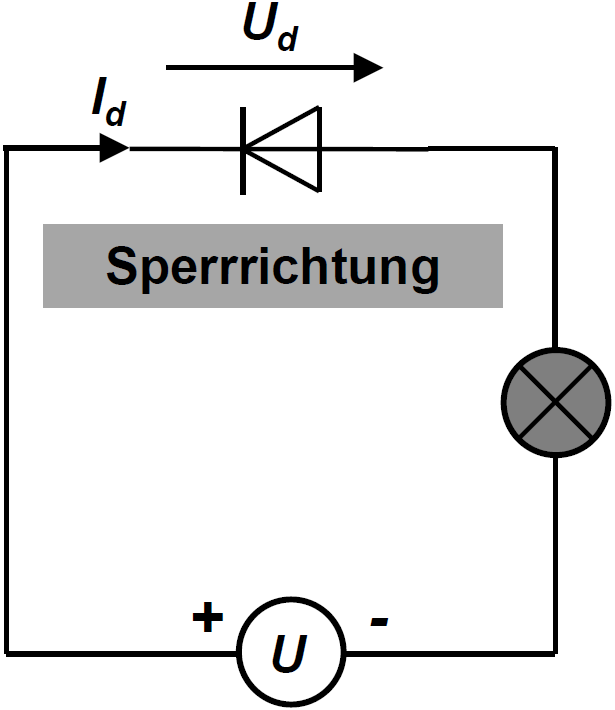
\includegraphics[width=0.75\columnwidth]{images/V2B0.png}
\end{minipage}
\hfill
\begin{minipage}[t]{0.49\columnwidth}
    \centering
    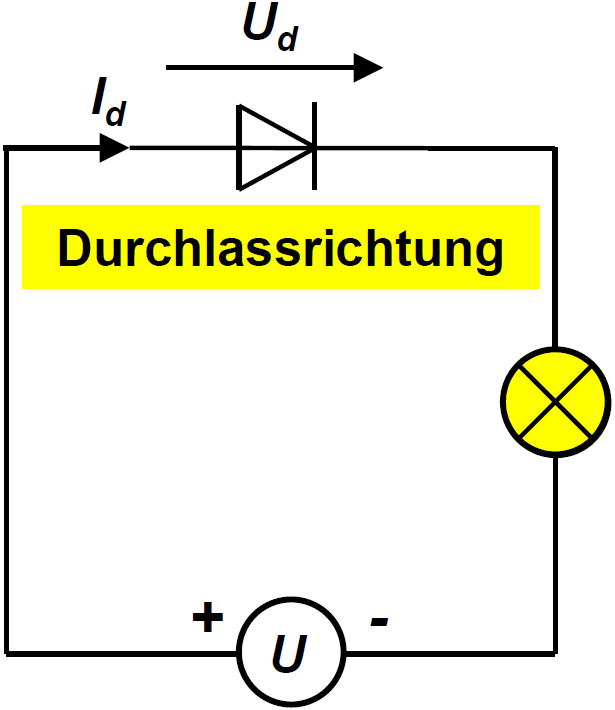
\includegraphics[width=0.75\columnwidth]{images/V2B1.png}
\end{minipage}
\\

\subsubsection{Kennlinie Diode}
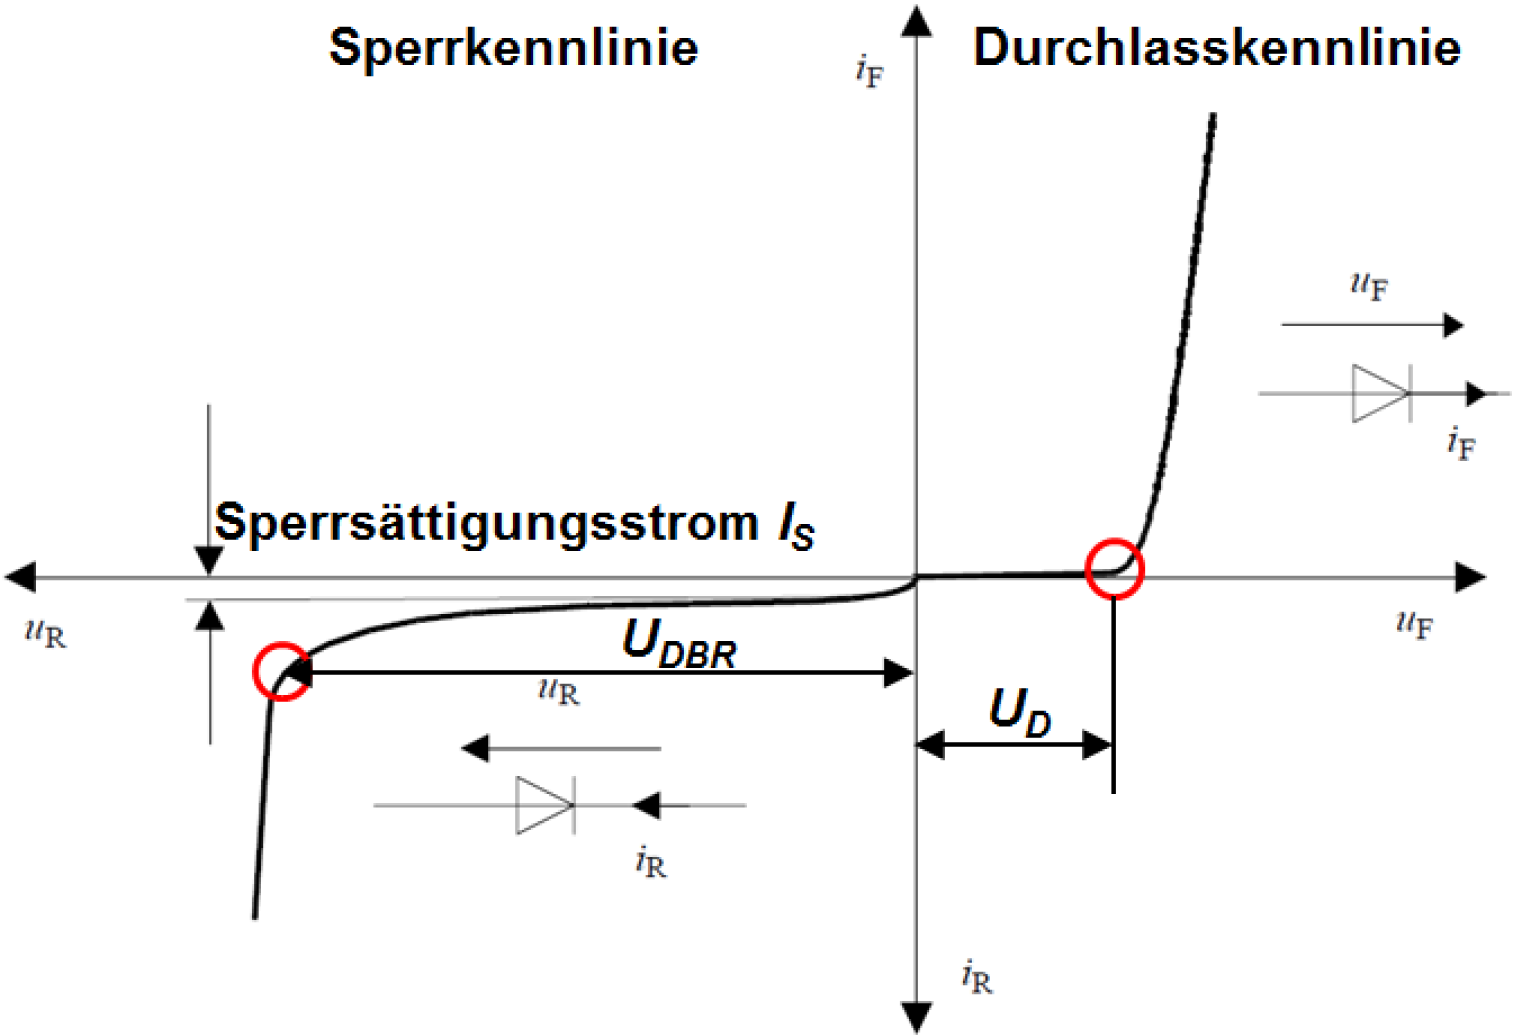
\includegraphics[width=0.95\columnwidth]{images/V2B2.png} \\

\begin{tabular}{lll}
    $u_{F}$ &=& Flussspannung (eng. forward voltage)\\
    $u_{R}$ &=& Sperrspannung (eng. reverse voltage)\\
    $U_{DBR}$ &=& Durchbruchspannung\\
    $i_{F}$ &=& Diffussionsstrom (eng. forward current)\\
            & & Strom in Durchlassrichtung\\
    $i_{R}$ &=& Leckstrom (eng. reverse current)\\
            & & Strom in Sperrrichtung\\
\end{tabular}
\\\\

\begin{minipage}[t]{1\columnwidth}
    \centering
    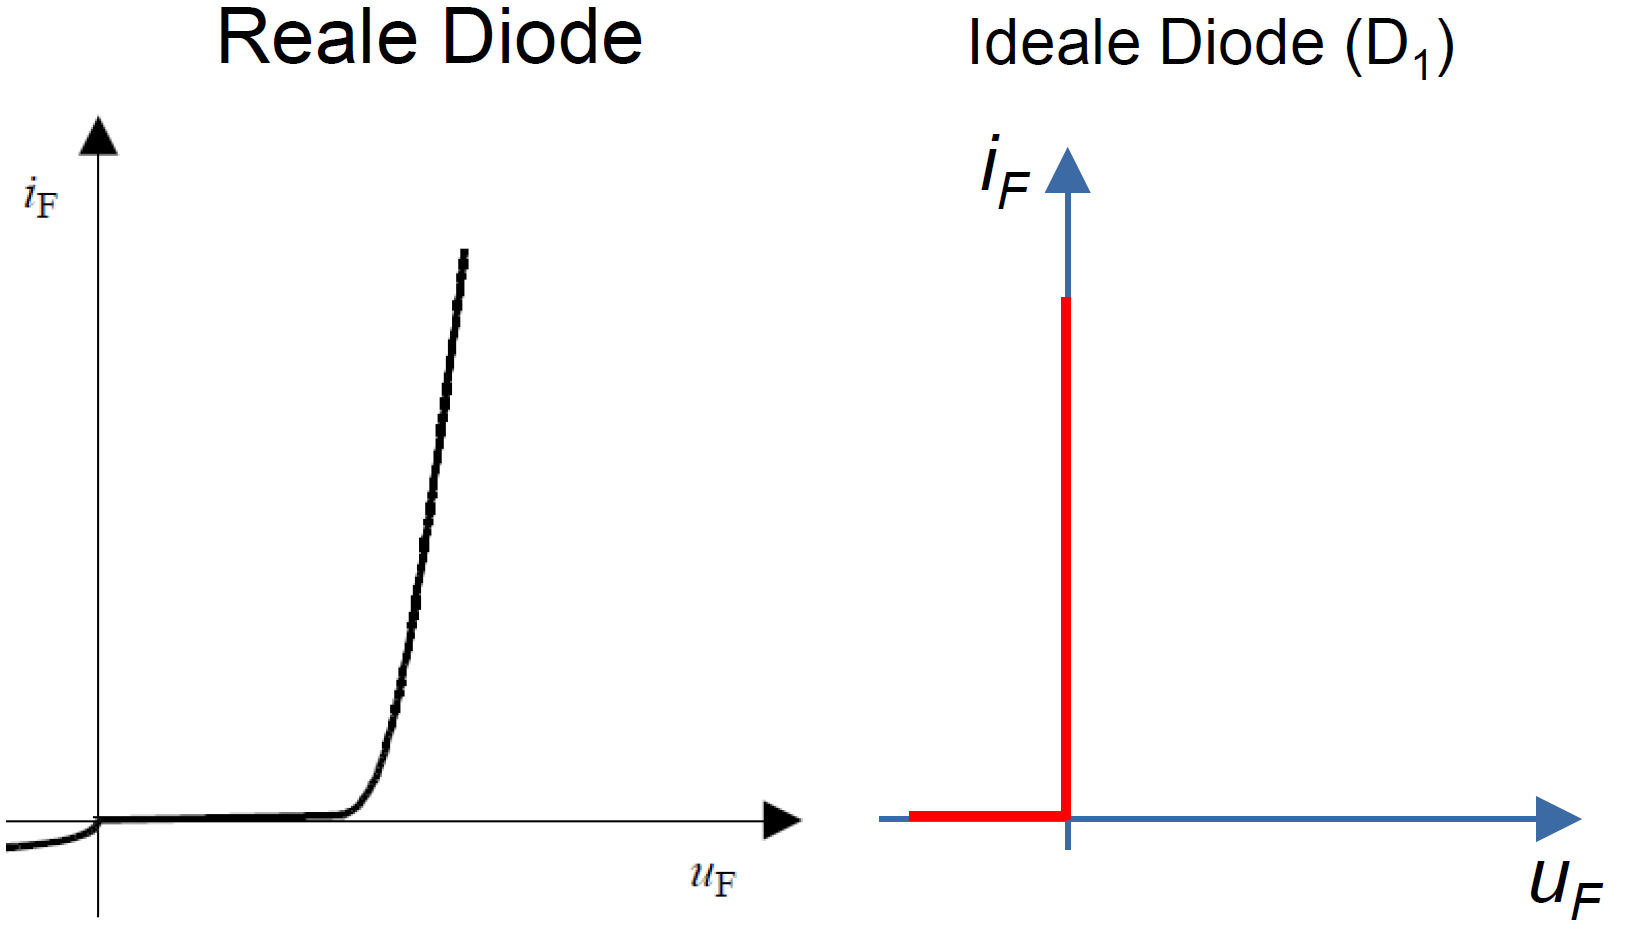
\includegraphics[width=0.9\columnwidth]{images/V2B4.png}\\
\end{minipage}
\begin{minipage}[t]{1\columnwidth}
    \centering
    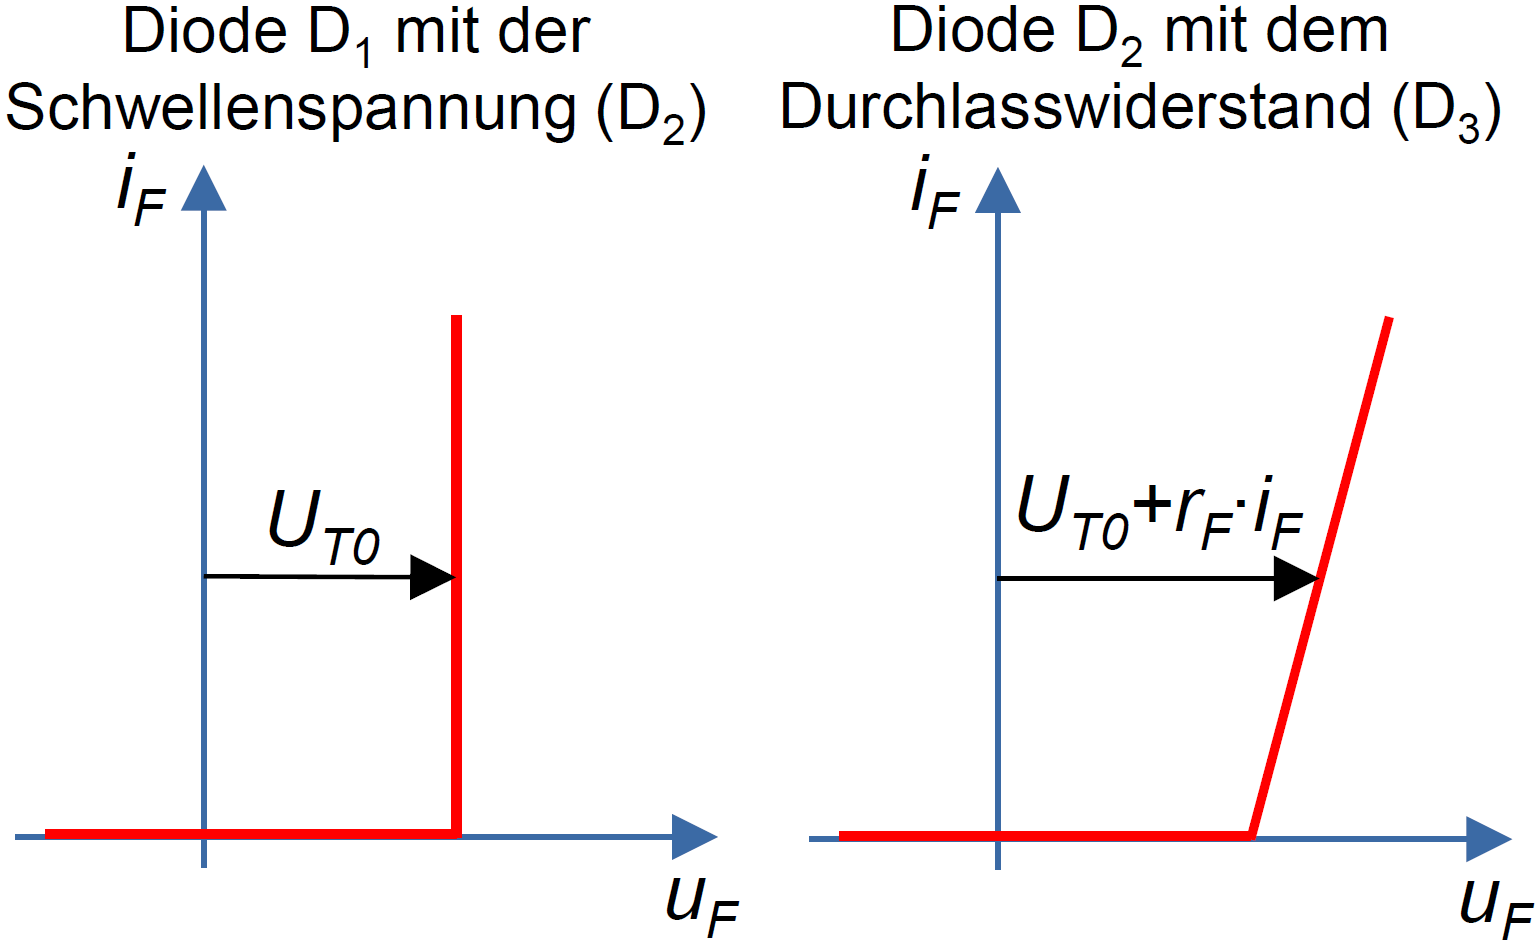
\includegraphics[width=0.9\columnwidth]{images/V2B5.png}\\
\end{minipage}


\subsubsection{Differenzieller Widerstand Diode}
\begin{minipage}[t]{0.49\columnwidth}
    \centering
    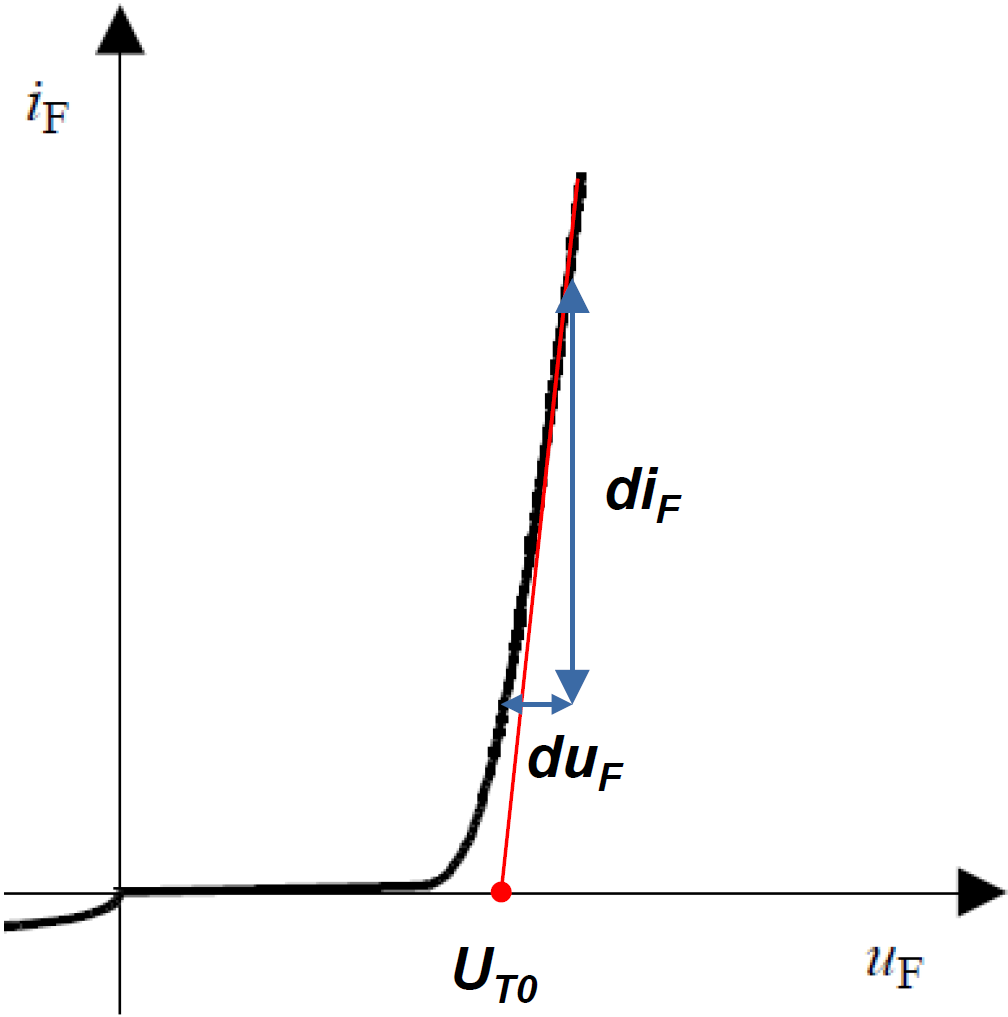
\includegraphics[width=0.85\columnwidth]{images/V2B3.png}
\end{minipage}
\hfill
\begin{minipage}[t]{0.49\columnwidth}
    $\boxed{u_F = U_{T_0} + i_F \cdot r_F }$ $\boxed{r_F = \frac{d u_F}{d i_F} }$    \\  
\end{minipage}

\begin{tabular}{lll}
    $u_{F}$ &=& Flussspannung (eng. forward voltage)\\

    $U_{T_0}$ &=& Schwellenspannung\\
    $i_{F}$ &=& Diffussionsstrom (eng. forward current)\\
            & & Strom in Durchlassrichtung\\
    $r_{F}$ &=& Differenzieller Widerstand\\
\end{tabular}


\subsubsection{Ersatzschaltbild Diode}

\begin{minipage}[t]{0.49\columnwidth}
    \centering
    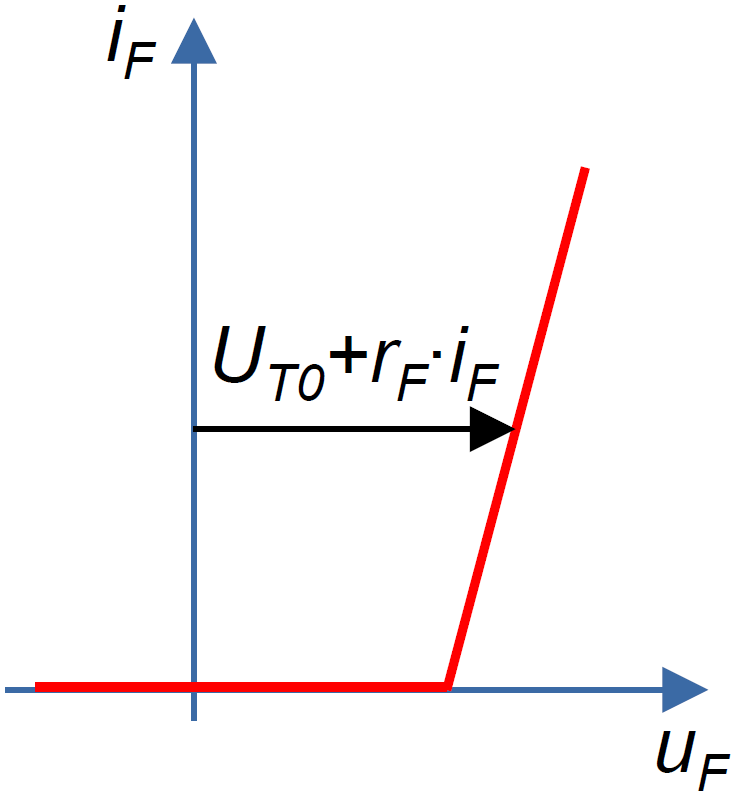
\includegraphics[width=0.95\columnwidth]{images/V2B6.1.png}
\end{minipage}
\hfill
\begin{minipage}[t]{0.49\columnwidth}
    \centering
    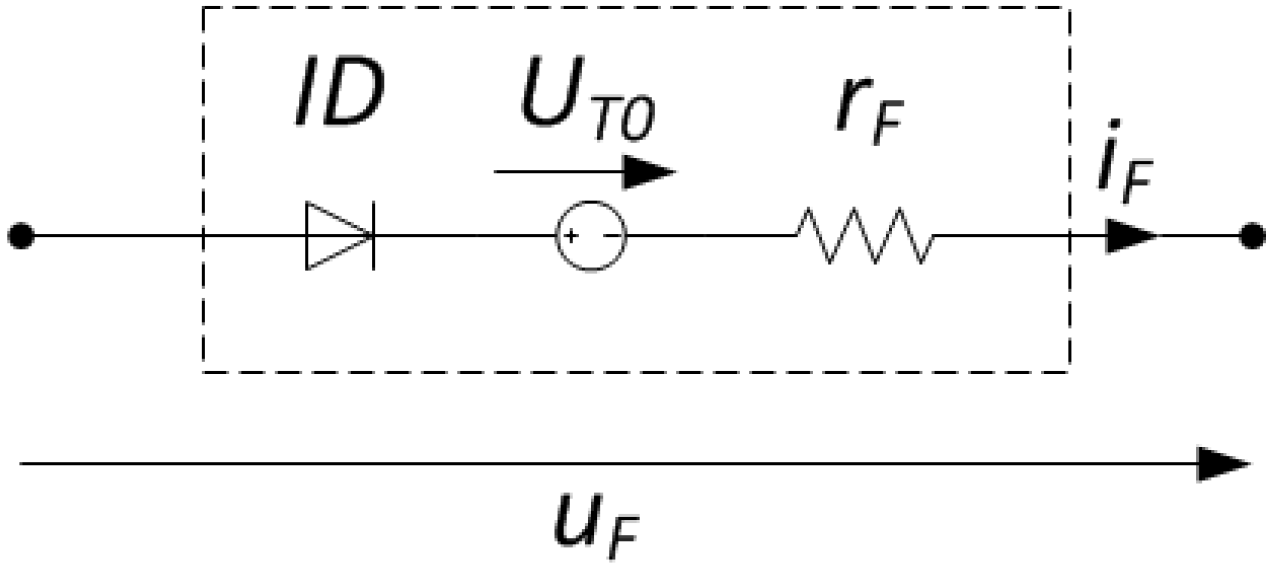
\includegraphics[width=0.95\columnwidth]{images/V2B6.png}
\end{minipage}

$\boxed{u_F = U_{T0} + i_F \cdot r_F }$\\

\begin{tabular}{lll}
    $u_{F}$ &=& Flussspannung (eng. forward voltage)\\

    $U_{T_0}$ &=& Schwellenspannung\\
    $i_{F}$ &=& Diffussionsstrom (eng. forward current)\\
            & & Strom in Durchlassrichtung\\
    $r_{F}$ &=& Differenzieller Widerstand\\
\end{tabular}


\subsubsection{Verlustleistungsberechung (Durchlassverluste) Diode}
\myul{Momantanleistung}\\\\
$\boxed{p(t) = u_F(t) \cdot i_F(t)}$\\

\myul{Verlustleistung}\\

$\boxed{P_V=\frac{1}{T}\int_0^Tu_F(t)\cdot i_F(t)\cdot dt}$\\

$\boxed{P_V = U_{T_0} \cdot \crd{I_{F_{AV}}} + r_F \cdot \cor{I_{F_{RMS}}}}$\\

$\boxed{P_V=U_{T_0} \cdot \crd{\frac{1}{T}\int_0^T i_F(t) \cdot dt} + r_F \cdot \cor{\frac{1}{T}\int_0^Ti_F^2(t)\cdot dt}}$\\

$\boxed{\crd{I_{F_{AV}}} = \frac{1}{T} \int_0^T i_F(t) \, dt}$\\

$\boxed{\cor{I_{F_{RMS}}} = \sqrt{\frac{1}{T} \int_0^T i^2_F(t) \, dt}}$\\

\begin{tabular}{lll}
    $p(t)$ &=& Momentanleistung\\
    $P_V$ &=& Verlustleistung\\
    $u_{F}$ &=& Flussspannung (eng. forward voltage)\\
    $U_{T_0}$ &=& Schwellenspannung\\
    $\crd{I_{F_{AV}}}$ &=& Arithmetischer Mittelwert des Stromes $i_F(t)$\\
    $\cor{I_{F_{RMS}}}$ &=& Effektivwert des Stromes $i_F(t)$\\
    $i_{F}$ &=& Diffussionsstrom (eng. forward current)\\
            & & Strom in Durchlassrichtung\\
    $r_{F}$ &=& Differenzieller Widerstand\\
\end{tabular}